%Marco Teórico

\section{Estimulación eléctrica funcional}
La estimulación eléctrica funcional es la aplicación de corriente eléctrica a tejido excitable para auxiliar o restaurar funciones que se han perdido en individuos con daños neurológicos. El propósito de la intervención FES es habilitar funciones que se han perdido en individuos con daño al sistema nervioso mediante la sustitución o asistencia a las habilidades voluntarias de dichos individuos. En las aplicaciones FES la estimulación es requerida para lograr una función deseada, por lo tanto, los sistemas FES usualmente se diseñan para ser controlados a partir de señales relacionadas a la actividad o intención del propio usuario. Los dispositivos FES que son usados para sustituir una función neurológica que se ha perdido son comúnmente llamados neuroprótesis \cite{Peckham2005}.

En la Figura \ref{Figura: FES} se puede observar que al aplicar estimulación eléctrica en el músculo, este responderá a dicha estimulación realizando una contracción, la cual puede ir disminuyendo durante el periodo de estimulación.

%Figura FES
\begin{figure}[htbp]
	\centering
	\begin{subfigure}[htbp]{0.4\textwidth}
		\centering
		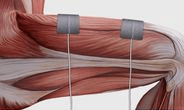
\includegraphics[width=\textwidth]{FES1.png}
		\caption{}
		\label{Figura: FES1}
	\end{subfigure}
	\hfill
	\begin{subfigure}[htbp]{0.4\textwidth}
		\centering
		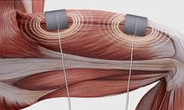
\includegraphics[width=\textwidth]{FES2.png}
		\caption{}
		\label{Figura: FES2}
	\end{subfigure}
	\caption[Efecto de aplicar estimulación eléctrica en músculo]{Efecto de aplicar estimulación eléctrica en músculo. (a) Músculo sin estimulación eléctrica. (b) Músculo con estimulación eléctrica. Recuperado de \cite{HASOMED}.}
	\label{Figura: FES}
\end{figure}

\section{Neuroprótesis}
Una neuroprótesis es un dispositivo compuesto de elementos que permiten utilizar la estimulación eléctrica como interface directa con el sistema nervioso, y cuyo fin es reemplazar o asistir alguna función deteriorada del sistema nervioso, deficiencia que suele ser el resultado de una enfermedad o lesión. Las neuroprótesis comúnmente actúan como un puente entre elementos funcionales del sistema nervioso central y los nervios o músculos sobre los cuales se ha perdido control (Figura \ref{Figura: NeuroP}) \cite{Finn2003}\cite{Popovic2008}.

%Una neuroprótesis es un dispositivo que proporciona ráfagas cortas de impulsos eléctricos al sistema nervioso central o periférico a través de electrodos superficiales, para lograr producir funciones sensoriales o motoras. Estos dispositivos buscan sustituir o asistir una función dañada debido a una lesión o enfermedad en el sistema nervioso \cite{Popovic2008} \cite{Popovic2015}.

En general, existen dos tipos de neuroprótesis: a) las neuroprótesis autónomas, las cuales son sistemas autocontenidos que imitan las funciones de una contraparte biológica, y b) las neuroprótesis por comando, las cuales son sistemas que reemplazan o asisten una función sensitiva o motora que se ha perdido o disminuido. Estas últimas están compuestos por un sistema de control que interpreta la intención del usuario, utilizan sensores para detectar el estado del sistema, genera la activación del sistema motor o sensorial del usuario, y proporciona una retroalimentación al usuario \cite{Popovic2015}.

Las neuroprótesis motoras, las cuales son un ejemplo de neuroprótesis por comando, son sistemas que asisten a personas que han sufrido algún tipo de lesión en la médula espinal o cerebro. Estas neuroprótesis pueden actuar directamente en el sistema nervioso central, en el sistema nervioso periférico, o bien, en una combinación de ambos, tiendo como objetivo principal realizar contracciones musculares que generen movimientos relevantes para el sujeto \cite{Popovic2015}.

%Figura Neuroprótesis
\begin{figure}[htbp]
	\centering
	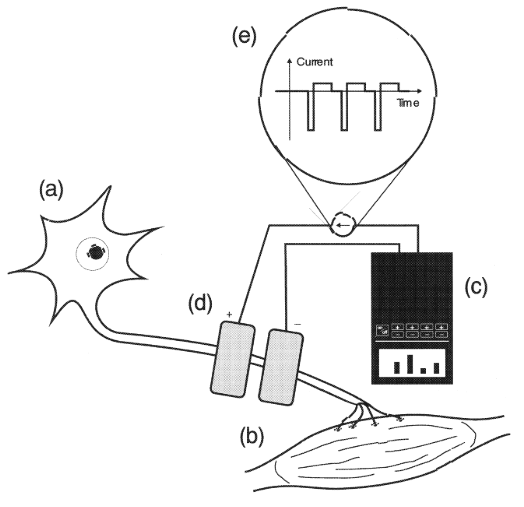
\includegraphics[width=0.4\textwidth]{NeuroP.png}
	\caption[Estimulación directa a una neurona motora]{Estimulación directa a una neurona motora. La neurona motora (a) es la responsable de generar señales de activación que son transmitidas a la correspondiente fibra muscular (b). Posterior a un accidente cerebrovascular o una lesión de la médula espinal, el músculo queda incomunicado con el sistema nervioso central. Una neuroprótesis (c) inyecta corriente eléctrica dentro del axón de la célula (d), corriente formada por un tren de pulsos negativos y positivos (e) que producen potenciales de acción que activan la fibra muscular. Recuperado de \cite{Popovic2008}.}
	\label{Figura: NeuroP}
\end{figure}

\section{Señales de comando y retroalimentación}\label{Seccion: ComRetro}

Una neuroprótesis por comando requiere de dos tipos de señales esenciales para lograr su correcto funcionamiento, las cuales son las señales de comando y las señales de retroalimentación \cite{Popovic2015}. En la Figura \ref{Figura: CompNeuroP} se pueden observar de forma general las conexiones que dichas señales realizan con el resto de los componentes de una neuroprótesis.

\begin{figure}[htbp]
\centering
	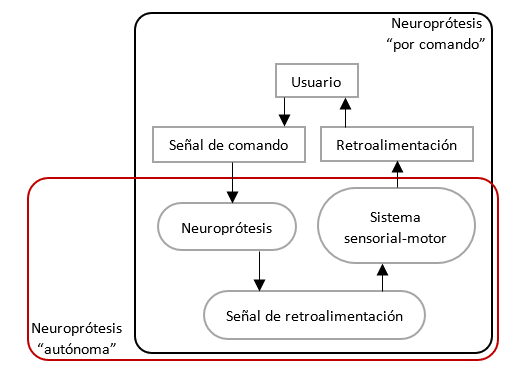
\includegraphics[width=0.6\textwidth]{CompNeuroP_ESP.png}
	\caption[Componentes generales de una neuroprótesis]{Componentes generales de una neuroprótesis autónoma (recuadro rojo) y por comando (recuadro negro). Adaptado de \cite{Popovic2015}.}
	\label{Figura: CompNeuroP}
\end{figure}

%\subsection{Señal de comando}
Las señales de comando son aquellas se usan para activar, desactivar o modular determinadas funciones o acciones dentro del sistema de control de la neuroprótesis. Estas señales pueden generarse de diversas formas, sin embargo, como se ilustra en la Figura \ref{Figura: CompNeuroP}, suelen ser generadas por el usuario \cite{Popovic2015}. Ejemplos de dichas señales podrían ser la acción de presionar un botón que indique a la neuroprótesis el momento de inicio y fin de la estimulación eléctrica; o bien, un conjunto de señales fisiológicas que permitan identificar la tarea que busca realizar el individuo.

%\subsection{Señal de retroalimentación}
En la Figura \ref{Figura: CompNeuroP} se puede observar que la señal de retroalimentación es aquella señal que se genera como salida de la neuroprótesis, es decir, la estimulación eléctrica que se inyecta al sistema sensorial-motor del usuario; sin embargo, también se puede observar una retroalimentación dirigida hacia el usuario, la cual hace referencia a la retroalimentación propioceptiva \cite{Popovic2015}. Esta última retroalimentación es la que suele ser relevante para el sistema de control de la neurorótesis.

Aclarado el concepto de retroalimentación que se abordará en el presente trabajo, se puede definir a las señales de retroalimentación como un tipo de señales que brindan información relacionada a la respuesta del sujeto ante un determinado comando. Dichas señales son útiles para indicar al sistema de control si la respuesta del sujeto se apega a la respuesta esperada, y en caso contrario modificar los parámetros de dicho sistema para conseguir la respuesta esperada \cite{Wright2016}. Estas señales de retroalimentación se pueden obtener de diversas maneras, las cuales se abordan en la sección \ref{Seccion: Retro}.

\section{Esquemas de control}
Existen dos tipos de control importantes dentro de las aplicaciones de una neuroprótesis, los cuales se diferencian esencialmente en los tipos de señales que ocupan. En la Figura \ref{Figura: EsqCont} se ilustran a grandes rasgos las diferencias entre ambos esquemas de control.

\begin{figure}[htbp]
\centering
	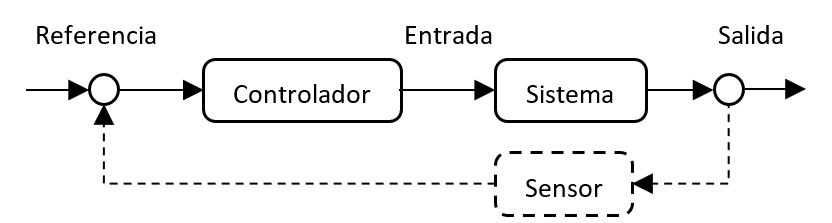
\includegraphics[scale=0.7]{EsquemasControl_ESP.png}
	\caption[Esquema general de control en lazo abierto y control en lazo cerrado]{Esquema general de control en lazo abierto y control en lazo cerrado. El control en lazo abierto se ilustra con una línea sólida. El control en lazo cerrado se lleva a cabo cuando se incluye el elemento sensor, el cual se ilustra con una línea discontinua. Adaptado de \cite{Wright2016}.}
	\label{Figura: EsqCont}
\end{figure}

%\subsection{Control en lazo abierto}
En el control en lazo abierto (línea sólida de la Figura \ref{Figura: EsqCont}) se genera un comando a la línea de base (estado o valor inicial del sistema), esperando que este comando produzca la salida correcta. Aquí no existe una medición de la salida generada, por lo cual tampoco existe alguna medición del error que pudiera utilizarse como mecanismo para la modulación del comando que se genera \cite{Wright2016}. En este esquema de control, los parámetros del sistema se encuentran predeterminados en base a consideraciones previas al experimento, y no sufren cambios durante la secuencia de estimulación.

%\subsection{Control en lazo cerrado}
El control en lazo cerrado (línea sólida más línea discontinua de la Figura \ref{Figura: EsqCont}) requiere de la inclusión de algún elemento sensor en el sistema que se desea controlar. Este control retroalimentado genera un comando a la línea de base y el elemento sensor mide la salida del sistema en respuesta al comando. Esta medición de la salida puede utilizarse para determinar diferencias entre la salida esperada y la real, generando así una señal de error que puede utilizarse como retroalimentación hacia el controlador para realizar modificaciones en los comandos generados \cite{Wright2016}.

%\subsection{Control adaptativo}
Otro esquema de control capaz de implementarse en aplicaciones de neuroprótesis (tanto en lazo abierto como en lazo cerrado) es el control adaptativo. Este esquema de control utiliza sensores para medir la entrada y salida del sistema, utilizando dichas métricas para ajustar el controlador en respuesta a las perturbaciones en el entorno de control o el sistema controlado, buscando siempre mantener un nivel de desempeño preestablecido. Una ventaja de este tipo de control es que se pueden desarrollar estrategias de control sin requerir de un conocimiento completo del sistema que se va a controlar, sin embargo, esto provoca que los controladores adaptativos rara vez sean óptimos \cite{Wright2016}.

\section{Algoritmos de control}
Existe una gran variedad de algoritmos de control que suelen ser usados dentro de las neuroprótesis, sin embargo, para este trabajo sólo se abordaran 3 algoritmos de control.

%\subsection{Control on-off}
El control on-off es un algoritmo que monitorea si una determinada variable de control se encuentra por encima o por debajo de un determinado umbral, con lo cual se suelen activar o desactivar determinadas funciones del sistema de control \cite{Wright2016}. En aplicaciones FES, este tipo de control suele utilizarse para activar una secuencia predefinida de estimulación eléctrica. Este algoritmo de control también suele utilizarse configurando dos umbrales por los cuales la variable de control puede pasar, por ejemplo, para el control de temperatura de una incubadora neonatal, en la cual se requiere que la temperatura de esta se encuentre dentro de un intervalo específico, en este caso, el control on-off podría aplicarse de la siguiente manera: si la temperatura se encuentra por encima del límite superior de temperatura, la calefacción se apaga; mientras que si la temperatura se encuentra por debajo del límite inferior de temperatura, la calefacción se enciende \cite{Wayne2003}.

%\subsection{Máquina de estados finitos (FSM)}
Una máquina de estados finitos (FSM, por sus siglas en inglés) es un modelo de sistema que puede considerarse como una implementación más compleja del control on-off. En este modelo, la medición de una variable del sistema en combinación con el estado actual de la misma, desencadenan una transición de estado, la cual a su vez genera una serie de acciones en el sistema que se está controlando. Debido a que este tipo de modelo suele ser periódico, puede ser útil para realizar transiciones de estado en respuesta al tiempo \cite{Wright2016}. En aplicaciones FES, las acciones generadas debido a la transición de estados suelen asociar al inicio o fin de la estimulación eléctrica, los periodos de rampa en el patrón de estimulación, o bien los periodos de modulación de la estimulación eléctrica.

%{\color{red}\subsection{Control proporcional}}
El control proporcional (también conocido como control P), es un tipo control en el cual se aplica una corrección a la variable de control, la cual es proporcional entre el valor deseado y el valor real. Este tipo de control es más complejo que el control on-off, pero a su vez es más simple que un control proporcional-integral-derivativo (PID). Este tipo de control suele ser útil para llevar a cabo el control de sistemas que cuentan con un tiempo de respuesta rápido. En este tipo de control, la salida es proporcional a la señal de error (diferencia entre el valor esperado y el real), proporción que está definida por la Ecuación \ref{Ecu: Recta}, donde $P$ representa la salida proporcional, $K_{p}$ representa la ganancia proporcional, $e(t)$ representa el error instantaneo en el momento $t$, $p_{0}$ representa la salida con cero errores \cite{Wayne2003}. En aplicaciones FES, este tipo de control se ha mostrado útil para llevar a cabo la modulación de algún parámetro de estimulación eléctrica (como puede ser la amplitud o el ancho de pulso), donde la determinación de los factores $K_{p}$ y $p_{0}$ serán los responsables directos del grado de desempeño de la modulación \cite{Zhou2018}.

\begin{equation}
	P = K_{p} e(t) + p_{0}
	\label{Ecu: Recta}
\end{equation}

\section{Retroalimentación}\label{Seccion: Retro}
Como se explicó en la sección \ref{Seccion: ComRetro}, una señal de retroalimentación es aquella que brinda información al sistema sobre los efectos ante un determinado comando. Estas señales se pueden implementar de más de una forma dentro de una neuroprótesis, por ejemplo, la observación visual de la acción realizado por algún actuador robótico de una una interfaz cerebro-computadora (comúnmente conocido como neurofeedback), la adquisición de una señal bioeléctrica durante un periodo de estimulación eléctrica, o bien la medición de algún elemento sensor que proporcione información sobre el estado del efector o actuador \cite{Wright2016}.

Otro ejemplo de retroalimentación en un sistema de neuroprótesis es el biofeedback, una técnica de retroalimentación donde no se requiere de elemento sensor en el efector o actuador del sistema, ya que consiste en permitir al individuo usuario de la neuroprótesis aprender a cambiar su actividad fisiológica con el fin de mejorar el rendimiento del sistema \cite{Yucha2008}.

\section{Electromiografía de superficie}
La electromiografía (EMG) es una técnica electrofisiológica mediante la cual se registra la señal eléctrica derivada de la actividad contráctil de los músculos. El EMG puede detectarse directamente mediante la inserción de electrodos en las fibras musculares, o de forma indirecta colocando electrodos de superficie en las zonas de la piel localizadas justo encima del tejido muscular. A este último método se le suele conocer como electromiografía de superficie (sEMG, por sus siglas en inglés), el cual, al ser un método de detección no invasivo y permitir obtener información sobre la activación muscular, como la intensidad de la contracción muscular, la manifestación de la fatiga muscular y el reclutamiento de unidades motoras, se ha convertido en un método muy popular en la investigación.

\subsection{Procesamiento del sEMG}
La actividad mioeléctrica en la superficie de la piel se encuentra dentro de un ancho de banda limitado que suele estar desde los 15 hasta los 400 Hz, con amplitudes dentro del rango de $\mu V$ o $mV$, dependiendo de la intensidad de la contracción muscular \cite{Cavalcanti-Garcia2009}.

La detección de la actividad mioeléctrica se realiza mediante el uso de un amplificador diferencial, el cual debe tener conectadas las entradas a un par de electrodos situados a lo largo de la dirección de la fibra muscular a sensar, y un tercer electrodo de referencia situado en el hueso más cercano a la fibra. Una vez detectada de forma eficaz la actividad mioeléctrica, esta debe someterse a un filtro analógico anti-aliasing y posteriorme al proceso de conversión analógico-digital que permitirá se realice el procesamiento digital de la señal \cite{Cavalcanti-Garcia2009}.

Usualmente se utilizan técnicas de procesamiento digital, como un filtro pasa banda con frecuencias de corte similares a las que componen la actividad mioeléctrica (15-400 Hz), acompañado de un filtro notch que permita atenuar la interferencia provocada por la línea \cite{Cavalcanti-Garcia2009}.

\subsection{Descriptores de amplitud del sEMG}
Existen diferentes indicadores que pueden ser utilizados para estimar la amplitud del sEMG, tal es el caso de la amplitud pico a pico, la cual nos proporciona un valor instantáneo de la amplitud del sEMG. Sin embargo, este no es un indicador robusto de la amplitud de la señal de sEMG \cite{Cavalcanti-Garcia2009}.

Los descriptores de amplitud de sEMG más comunes son la promediación de muestras rectificadas o elevadas al cuadrado de sEMG crudo a lo largo de una determinada tarea motora. Estos descriptores se conocen como el valor rectificado promedio (ARV o MAV, por sus siglas en inglés)(Ecuación \ref{Ecu: ARV}) y el valor cuadrático medio (RMS, pos sus siglas en inglés)(Ecuación \ref{Ecu: RMS}). Dichos descriptores suelen usarse para estimar las variaciones temporales de la amplitud del sEMG en ventanas cortas entre 250 ms o 500 ms \cite{Cavalcanti-Garcia2009}.

\begin{equation}
	ARV = \frac{1}{N} \sum_{n=1}^{N} \abs{EMG[n]}
	\label{Ecu: ARV}
\end{equation}

\begin{equation}
	RMS = \sqrt{\frac{1}{N} \sum_{n=1}^{N} EMG[n]^{2}}
	\label{Ecu: RMS}
\end{equation}

Estos descriptores de amplitud suelen proporcionar información similiar, la gran diferencia entre ellos se encuentra en la función de densidad de probabilidad (PDF, por sus siglas en inglés) que generan, donde el RMS suele ser un descriptor con PDF Gaussiana, mientras que el ARV suele ser una descriptor con PDF Laplaciana. En general, se suele utilizar el RMS debido que teóricamente la PDF del sEMG es gaussiana, sin embargo, existen trabajos que han demostrado que en la práctica la PDF del sEMG es más cercana a una PDF laplaciana, en cuyo caso es recomendable utilizar el ARV como descriptor \cite{Clancy1999}\cite{Phinyomark2013}.